\appendix
\chapter{Apéndices}

\section{Resultados algoritmo DMRG}
\label{apendix:dmrg}

En este apéndice presentamos resultados numéricos del funcionamiento del algoritmo DMRG. El problema a resolver por el algoritmo DMRG es el problema Max Cut, presentado en el apartado \ref{sub:problem_target}. La calidad del resultado obtenido por el algoritmo DMRG depende del numero de pasos de optimización realizados y de la dimensión interna considerada para mapear el Hamiltoniano en un MPO así como la dimensión interna máxima permitida para representar el estado solución en un MPS. Tal y como puede verse en la Figura \ref{fig:result_dmrg}, la calidad de la solución obtenida depende de la dimensión interna $\chi$ que posee tanto el MPO como el MPS que participa en el proceso de optimización.

\begin{figure}[!h]
    \centering
    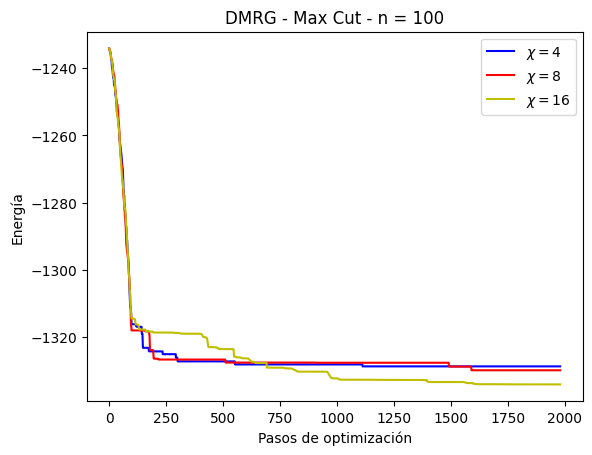
\includegraphics[scale = 0.7]{plt/a01-dmrg_max_cut_n_100.png}
    \caption{resultados DMRG problema Max Cut para 100 nodos}
    \label{fig:result_dmrg}
\end{figure}

Con pocos pasos de optimización, la calidad de la solución obtenida puede ser mejor con un $\chi$ bajo, dado que el subespacio de Hilbert en el que busca el algoritmo DMRG es menor y por lo tanto encuentra antes cual es el estado $\psi$ de ese subespacio que minimiza la energía del MPO. 

\newpage

\section{Resultados de los algoritmos de traducción}
\label{apendix:mps_to_pqc}

En este apéndice se presentan resultados orientados a mostrar las particularidades de los algoritmos de traducción de MPS a PQC.

\subsection{Traducción analítica}

El protocolo de traducción analítica permite construir cada capa de operadores unitarios de dos qubits en base a unas reglas fijas. Estas reglas permiten construir los tensores $G$ de dos qubits los cuales tienen una correspondencia directa con operadores de dos qubits, tal y como se observa en la Figura \ref{fig:mpd_to_pqc}. Las reglas las cuales permiten construir los tensores $G$ a partir de los tensores $A$ pertenecientes al MPS de $\chi =2$ vienen dado por el conjunto de expresiones \ref{eq:rules_mps_to_pqc}.

\begin{equation}
\begin{aligned}
G^{[8]} &= A^{[8]} \\
G_{00kl}^{[1]} &= A_{kl}^{[1]} \\
G_{0jkl}^{[n]} &= A_{jkl}^{[n]} \\
\sum_{kl} G^{[n]}_{i^{'} j^{'} k l} G^{[n]*}_{i j k l} &= I_{i^{'} i} I_{j^{'} j}
\end{aligned}
\label{eq:rules_mps_to_pqc}
\end{equation}

El protocolo de traducción analitico aún siendo eficiente en terminos de coste computacional, arroja resultados poco precisos cuando la dimesión $\chi$ del MPS que se desea replicar crece.


\begin{figure}[!h]
    \centering
    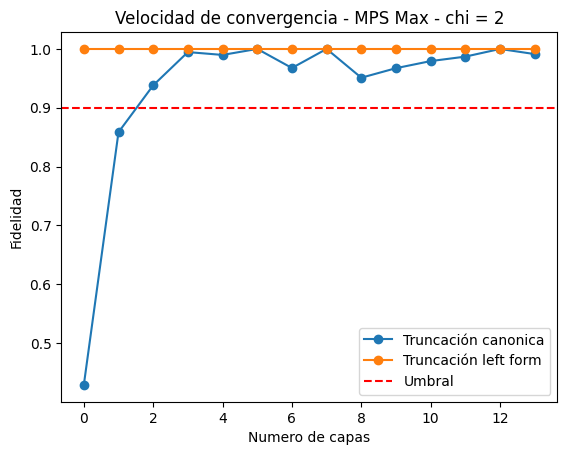
\includegraphics[scale = 0.6]{plt/a02-mps_to_pqc_a.png}
    \caption{resultados del proceso de traducción analítica de un MPS de $\chi = 2$ a PQC}
    \label{fig:r_mps_to_pqc_a}
\end{figure}

\newpage

Tal y como se puede observar en la Figura \ref{fig:r_mps_to_pqc_a}, con un MPS inicial de $\chi = 2$, existen inestabilidades numéricas asociadas a la metodología  \textit{canónica} la cual requiere de mas capas para poder replicar un MPS de $\chi = 2$, cuando idealmente solo necesita una, tal y como ocurre con el método \textit{left form}. El umbral marca la fidelidad a partir del cual podemos detener el proceso de traducción. Por otro lado, cuando se intenta traducir a un PQC, un MPS de $\chi > 2$ encontramos que las inestabilidades numéricas lo impiden, tal y como puede verse en la Figura \ref{fig:r_mps_to_pqc_a_2}.


\begin{figure}[!h]
    \centering
    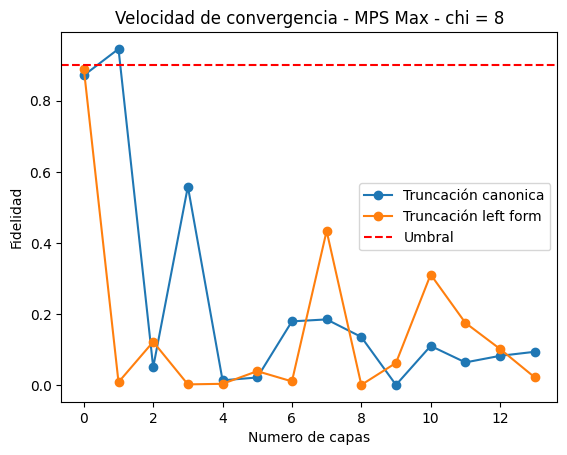
\includegraphics[scale = 0.7]{plt/a03-mps_to_pqc_a_2.png}
    \caption{resultados del proceso de traducción analítica de un MPS de $\chi = 8$ a PQC}
    \label{fig:r_mps_to_pqc_a_2}
\end{figure}

En \ref{fig:r_mps_to_pqc_a_2} se observa como mayor numero de capas no garantiza una mejora en la fidelidad conseguida entre el MPS inicial y el PQC generado.

\subsection{Traducción por optimización}

El método de traducción por optimización de MPS a PQC siendo mas costoso computacionalmente genera resultados los cuales son mas consistentes y precisos. Tal y como puede observarse en la Figura \ref{fig:r_mps_to_pqc_o} el algoritmo de traducción por optimización consigue replicar un MPS de $\chi = 64$ con tan solo 2 y 4 capas de un PQC. En general se puede replicar un MPS, si este contiene solo coeficientes reales, de $\chi = n$ con un PQC que tenga, en terminos de $\chi$, un valor menor. Cada capa de PQC, implica un aumento de \textit{x4} en el aumento de $\chi$, de tal forma que un PQC de dos capas generan un MPS de $\chi = 16$.

\newpage

\begin{figure}[!h]
    \centering
    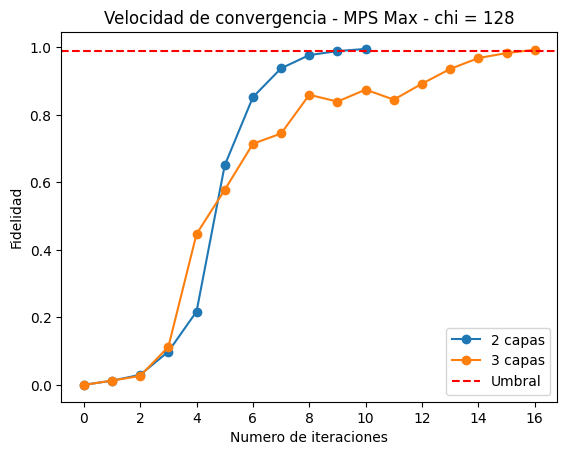
\includegraphics[scale = 0.7]{plt/a04-mps_to_pqc_o.png}
    \caption{resultados del proceso de traducción por optimización de un MPS de $\chi = 128$ a PQC}
    \label{fig:r_mps_to_pqc_o}
\end{figure}

La propiedad de replicar estados de MPS en PQC's de dimesión $\chi$ inferior es utilizada en algoritmos ciertos algoritmos de compresión.

\section{Resultados algoritmo MPO Time Evolution}
\label{apendix:mpo_time_evolution}

En este apéndice presentamos resultados numéricos del funcionamiento del algoritmo MPO Time Evolution. El MPO Time evolution es usado para implementar la evolución temporal imaginaria del sistema cuántico. El problema a resolver por el algoritmo MPO Time Evolution, al igual que el algoritmo DMRG, es el problema Max Cut, presentado en el apartado \ref{sub:problem_target}. De forma análoga al algoritmo DMRG, la calidad de la solución obtenida por el algoritmo MPO Time Evolution depende del tiempo de evolución durante el cual se hace evolucionar al sistema, así como la discretización $\delta \tau$ utilizada, y de la dimesión interna $\chi$ máxima permitida tanto para el MPS, que representa el estado cuántico, como para el MPO, que representa el Hamiltoniano. En la Figura \ref{fig:result_tevo} se puede observar como la calidad de la solución encontrada está influida fuertemente por la discretización del tiempo usada. Es importante recordar que el error asociado al MPO Time evolution es del orden de $(\delta \tau)^2$, lo cual limita no solo la calidad de la solución encontrada si no también la calidad del estado de Gibbs puro construido.

\newpage

\begin{figure}[!h]
    \centering
    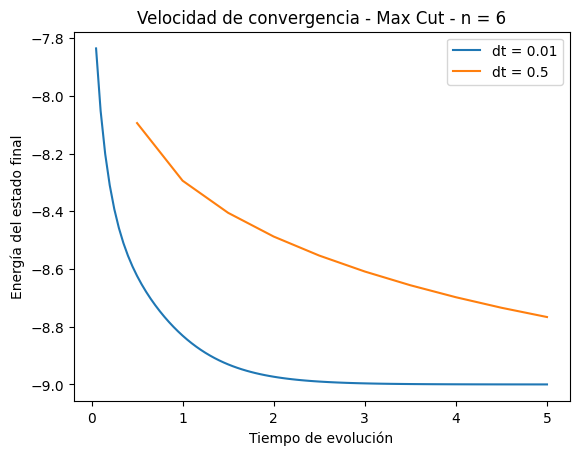
\includegraphics[scale = 0.7]{plt/a05-tevo_max_cut_n_6.png}
    \caption{resultados MPO Time Evolution para un Max Cut de 6 nodos}
    \label{fig:result_tevo}
\end{figure}

Es importante demostrar que los estados construidos son realmente estados de Gibbs de la temperatura esperada. Para comprobar que los estados generados son realmente estados de Gibbs podemos utilizar el hecho de conocer cual es la distribución de probabilidad esperada. Se sabe que los coeficientes de un estado de Gibbs puro viene dado por la expresión \ref{eq:coeficient_gibbs}.

\begin{equation}
c_{i} = \frac{e^{- \frac{E_{i}}{T}}}{Q}
\label{eq:coeficient_gibbs}
\end{equation}

Donde el factor $Q$ representa la constante de normalización del estado, $T$ la temperatura asociada y $E_{i}$ la energía asociado al autoestado del Hamiltoniano $\ket{i}$. Tomando el logaritmo en base $e$ de la expresión \ref{eq:coeficient_gibbs} obtenemos la expresión \ref{eq:coeficient_gibbs_log}.

\begin{equation}
\log(c_{i}) = \frac{- E_{i}}{T} - \log(Q)
\label{eq:coeficient_gibbs_log}
\end{equation}

Dada la forma de la expresión \ref{eq:coeficient_gibbs_log}, si se representa la energía como valor $x$ de una función y el logaritmo de $c_{i}$ como el valor $y$ de la función, debemos esperar que la función será una recta de pendiente $-\frac{1}{T}$. Esto es lo que se ha representado en la Figura \ref{fig:result_gibbs_pb}, para comprobar que el algoritmo MPO Time Evolution implementa correctamente los estados de Gibbs puros.

\newpage

\begin{figure}[!h]
    \centering
    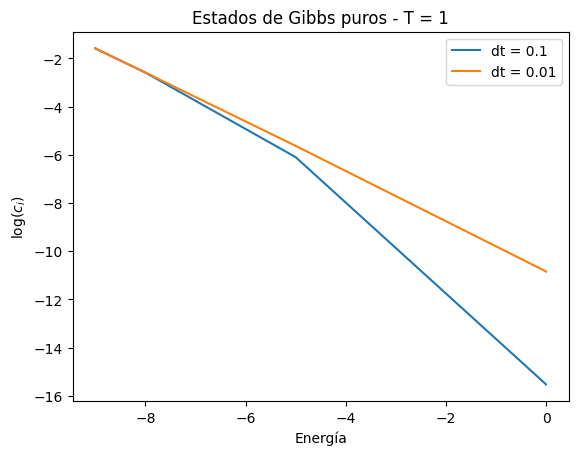
\includegraphics[scale = 0.7]{plt/a06-gibbs_state_pb.png}
    \caption{distribución de probabilidad para un estado de Gibbs puro de $T=1$}
    \label{fig:result_gibbs_pb}
\end{figure}

Para la Figura \ref{fig:result_gibbs_pb} se puede observar como la pendiente de la recta posee valor $p=-1$, que es la temperatura esperada del estado de Gibbs.

\section{Análisis del campo de energías}
\label{apendix:energy_landscape}

Una forma de intentar descubrir por que los estados de Gibbs maximizan el rendimiento del algoritmo QAOA es mediante un análisis del campo de energías en el cual algoritmo QAOA trata de encontrar el mínimo global. El algoritmo QAOA formando por una sola capa, contiene dos operadores parametrizados, cada uno de ellos con ángulo a optimizar, tal y como se ve en la expresión \ref{eq:pqc_qaoa_one_layer}.


\begin{equation}
    U(\gamma,\beta)= e^{-i \gamma H_C} e^{- i \beta H_M}
    \label{eq:pqc_qaoa_one_layer}
\end{equation}

Dado el QAOA formado por una sola capa, a traves del operador de la expresión \ref{eq:pqc_qaoa_one_layer}, que posee solo dos parámetros, podemos visualizar directamente el campo de energías. En la Figura \ref{fig:landscape_energy} se muestra cual es el campo de energías que genera el algoritmo QAOA de una sola capa para un problema concreto de Max Cut de $N=7$. El estado de Gibbs y el estado de pseudoGibbs poseen la misma energía pero el estado de pseudoGibbs contiene ligeramente menor entropía. 

\newpage

Los ejes $x$ e $y$ de ambos gráficos hacen referencia al valor que toman los parámetros $\alpha$ y $\beta$. El código de colores hace referencia al valor esperado energía que se obtiene cuando se ejecuta el QAOA con los valores de $\alpha$ y $\beta$ correspondientes.

\begin{figure}[!h]
    \centering
    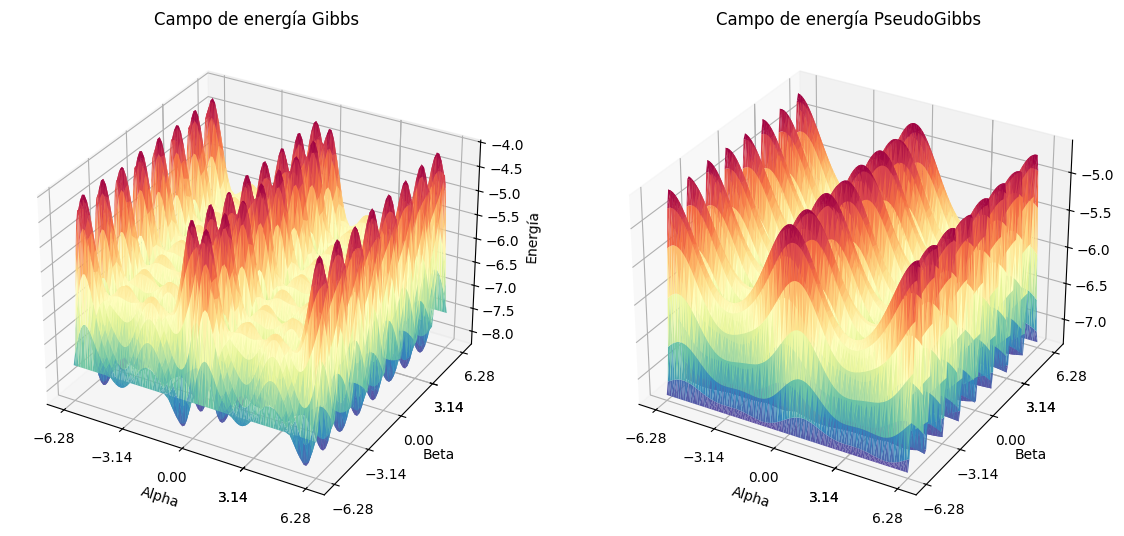
\includegraphics[scale = 0.55]{plt/a07-energy_landscape.png}
    \caption{campos de energías para estados de Gibbs y de pseudoGibbs de igual energía}
    \label{fig:landscape_energy}
\end{figure}

En la Figura \ref{fig:landscape_energy} puede observarse como el estado de Gibbs mejora la expresividad del circuito QAOA permitiendo encontrar mínimos globales mas profundos, a diferencia del circuito QAOA inicializado con el estado de pseudoGibbs. La mejorar del rendimiento del algoritmo QAOA cuando se utilizan estados de Gibbs puros como estados de inicialización puede deberse en parte al hecho de que se mejora la expresividad del circuito QAOA.